\documentclass[12pt]{article}
\usepackage[english]{babel}
\usepackage{natbib}
\usepackage{url}
\usepackage[utf8x]{inputenc}
% https://tex.stackexchange.com/questions/9866/latest-advice-on-the-euro-symbol
\usepackage{lmodern,textcomp}
\usepackage{amsmath}
\usepackage{amsthm}
\usepackage{graphicx}
% https://www.overleaf.com/learn/latex/How_to_Write_a_Thesis_in_LaTeX_(Part_3):_Figures,_Subfigures_and_Tables
\usepackage{caption}
\usepackage{subcaption}
\graphicspath{{images/}}
\usepackage{parskip}
\usepackage{fancyhdr}
\usepackage{vmargin}
\setmarginsrb{3 cm}{2.5 cm}{3 cm}{2.5 cm}{1 cm}{1.5 cm}{1 cm}{1.5 cm}
%https://tex.stackexchange.com/questions/60209/how-to-add-an-extra-level-of-sections-with-headings-below-subsubsection
\usepackage{titlesec}

% Allows usage of [H] in \begin{figure}
\usepackage{float}

% Define custom colors, for example for highlighting filenames
\usepackage{xcolor}
\definecolor{light-gray}{gray}{0.95}

% Links in table of contents
\usepackage{hyperref}
\hypersetup{
	colorlinks=true, %set true if you want colored links
	linktoc=all,     %set to all if you want both sections and subsections linked
	linkcolor=blue,  %choose some color if you want links to stand out
}

% https://tex.stackexchange.com/questions/10684/vertical-space-in-lists
% https://tex.stackexchange.com/questions/2291/how-do-i-change-the-enumerate-list-format-to-use-letters-instead-of-the-defaul
\usepackage[shortlabels]{enumitem}
\setlist{nosep}

% Color boxes
% https://ctan.org/pkg/tcolorbox
\usepackage{tcolorbox}

% For the R for real numbers and other symbols
\usepackage{amssymb}

% https://tex.stackexchange.com/questions/439768/put-reference-above-equal-sign-and-refer-to-it
\newcommand\numeq[1]%
{\stackrel{\scriptscriptstyle(\mkern-1.5mu#1\mkern-1.5mu)}{=}}

% https://tex.stackexchange.com/questions/7350/how-do-i-add-dots-in-toc
\usepackage{tocloft}
\renewcommand{\cftsecleader}{\cftdotfill{\cftdotsep}}

% https://tex.stackexchange.com/questions/28836/typesetting-the-define-equals-symbol
\usepackage{mathtools}
\newcommand{\defeq}{\vcentcolon=}
\newcommand{\eqdef}{=\vcentcolon}

% https://tex.stackexchange.com/questions/159257/increase-latex-table-row-height
{\renewcommand{\arraystretch}{2}

% https://www.overleaf.com/learn/latex/Environments
\theoremstyle{definition}
\newtheorem{example}{Example}[section]
\theoremstyle{definition}
\newtheorem{definition}{Definition}[section]
\theoremstyle{theorem}
\newtheorem{theorem}{Theorem}

%%%%%%%%%%%%%%%%%%%%%%%%%%%%%%%%%%%%%%%%%%%%%%%%%%%%%%%%%%%%%%%%%%%%%%%


\title{Handbook of Statistics}
\author{David Silva Sanmartín}
\date{\today}

\makeatletter
\let\thetitle\@title
\let\theauthor\@author
\let\thedate\@date
\makeatother

\pagestyle{fancy}
\fancyhf{}
\rhead{\theauthor}
\lhead{\thetitle}
\cfoot{\thepage}

\begin{document}

	% Make all the references appear always
	\nocite{*}

	%%%%%%%%%%%%%%%%%%%%%%%%%%%%%%%%%%%%%%%%%%%%%%%%%%%%%%%%%%%%%%%%%%%%%%%%%%%%%%%%%%%%%%%%%
	
	\begin{titlepage}
		\centering
		\vspace*{0.5 cm}
		
\includegraphics[scale = 0.2]{uned.jpg}\\[1.0 cm] % University Logo
		\textsc{\LARGE Mathematics}\\[2.0 cm] % University Name
		%\textsc{\Large Modelización}\\[0.5 cm] % Course Code
		%\textsc{\large Herramientas Informáticas Para Matemáticas}\\[0.5 cm] % Course Name
		\rule{\linewidth}{0.2 mm} \\[0.4 cm]
		{ \huge \bfseries \thetitle}\\
		\rule{\linewidth}{0.2 mm} \\[1.5 cm]
		
		\begin{minipage}{0.4\textwidth}
			\begin{flushleft} \large
				\emph{Author:}\\
				\theauthor
			\end{flushleft}
		\end{minipage}~
		\begin{minipage}{0.4\textwidth}
			\begin{flushright} \large
			\end{flushright}
		\end{minipage}\\[2 cm]
		
		{\large \thedate}\\[2 cm]
		
		\vfill
		
	\end{titlepage}
	
	%%%%%%%%%%%%%%%%%%%%%%%%%%%%%%%%%%%%%%%%%%%%%%%%%%%%%%%%%%%%%%%%%%%%%%%%%%%%%%%%%%%%%%%%%
	
	\tableofcontents
	\pagebreak
	
	%%%%%%%%%%%%%%%%%%%%%%%%%%%%%%%%%%%%%%%%%%%%%%%%%%%%%%%%%%%%%%%%%%%%%%%%%%%%%%%%%%%%%%%%%
	
	\section{Definitions}
	\subsection{Random variables and expectations}
\begin{definition}
	\textbf{Random Experiment:} an experiment whose outcomes are determined only by chance factors.
\end{definition}
\begin{definition}
	\textbf{Sample Space:} the set of all possible outcomes of a random experiment.
\end{definition}
\begin{definition}
	\textbf{Event:} the collection of none, one, or more than one outcomes from a sample space.
\end{definition}
\begin{definition}
	\textbf{Random Variable}: a variable whose numerical values are determined by chance factors. It is a function from the sample space to a set of real numbers.
\end{definition}
\begin{definition}
	\textbf{Discrete Random Variable:} if the set of all possible values of a random variable $X$ is countable, then $X$ is called a \textit{discrete random variable}.
\end{definition}
\begin{definition}
	\textbf{Probability Mass Function (pmf):} let $R$ be the set of all possible values of a random variable $X$, and $f(k) = P(X = k)$ for each $k$ in $R$. Then $f(k)$ is called the \textit{probability mass function} of $X$.
\end{definition}
\begin{definition}
	\textbf{Continuous Random Variable:} if the set of all possible values of $X$ an interval or union of two or more nonoverlapping intervals in $\mathbb{R}$, then $X$ is called a \textit{continuous random variable}.
\end{definition}
\begin{definition}
	\textbf{Probability Density Function (pdf):} any real valued function $f(x)$ that satisfies the following requirements is called a \textit{probability density function}:
	\[
		f(x) \geq 0 \text{ for all } x, \text{ and } \int_{-\infty}^{\infty}f(x)\,dx = 1
	\]
\end{definition}
\begin{definition}
	\textbf{Cumulative Distribution function (pdf):}
\end{definition}
\begin{definition}
	\textbf{}
\end{definition}
\begin{definition}
	\textbf{}
\end{definition}
\begin{definition}
	\textbf{}
\end{definition}
\begin{definition}
	\textbf{}
\end{definition}

	
	\section{Discrete uniform distribution}
	%\begin{figure}[H]
%	\centering
%	\includegraphics[width=\textwidth]{pr0201.png}
%\end{figure}
\subsection{Description}
Used to model experimental outcomes which are "equally likely".

\subsubsection{Probability mass function}
$$P(X=k)=\frac{1}{N},\quad k=1,\ldots,N$$

\subsubsection{Cumulative distribution function}
$$P(X \leq k)=\frac{k}{N},\quad k=1,\ldots,N$$

\subsubsection{Plot}

\subsection{Moments}
\begin{center}
	\begin{tabular}{l l}
		Mean & $\frac{N+1}{2}$ \\
		Variance & $\frac{(N-1)(N+1)}{2}$\\
	\end{tabular}
\end{center}

	
	\section{Binomial distribution}
	\section{Description}

A binomial experiment involves $n$ independent and identical trial such that each trial can result into one of the two possible outcomes: success of failure. If $p$ is the probability of observing success in each trial, then the number of successes $X$ that can be observed out of these $n$ trials is referred to as the \textbf{binomial random variable with $n$ trials and success probability $p$}, or $B(n, p)$.

Binomial distribution is often used to estimate or determine the proportion of individuals with a particular attribute in a large population. Suppose that a random sample of $n$ units is drawn by sampling with replacement from a finite population or by sampling without replacement from a large population. The number of units that contain the attribute of interest in the sample follows a normal distribution.

If the sample was drawn without replacement from a small finite population, the hypergeometric distribution should be used instead of the binomial.

\subsection{Probability mass function}
The probability of observing $k$ successes out of $n$ trials is given by the following probability mass function
\[
	P(X = k \mid n, p) = \binom{n}{k}p^{k}(1 - p)^{n - k}, \quad k = 0, 1, \ldots, n
\]

Binomial's pmf is right-skewed when $p < 0.5$, left-skewed when $p > 0.5$ and symmetric when $p = 0.5$.

% For the future: on image and floats positioning
% https://tex.stackexchange.com/questions/278727/split-subfigures-over-multiple-pages/278748
% https://tex.stackexchange.com/questions/16207/image-from-includegraphics-showing-up-in-wrong-location/16211
\begin{figure}[H]
	\centering
	\begin{subfigure}[b]{0.45\textwidth}
		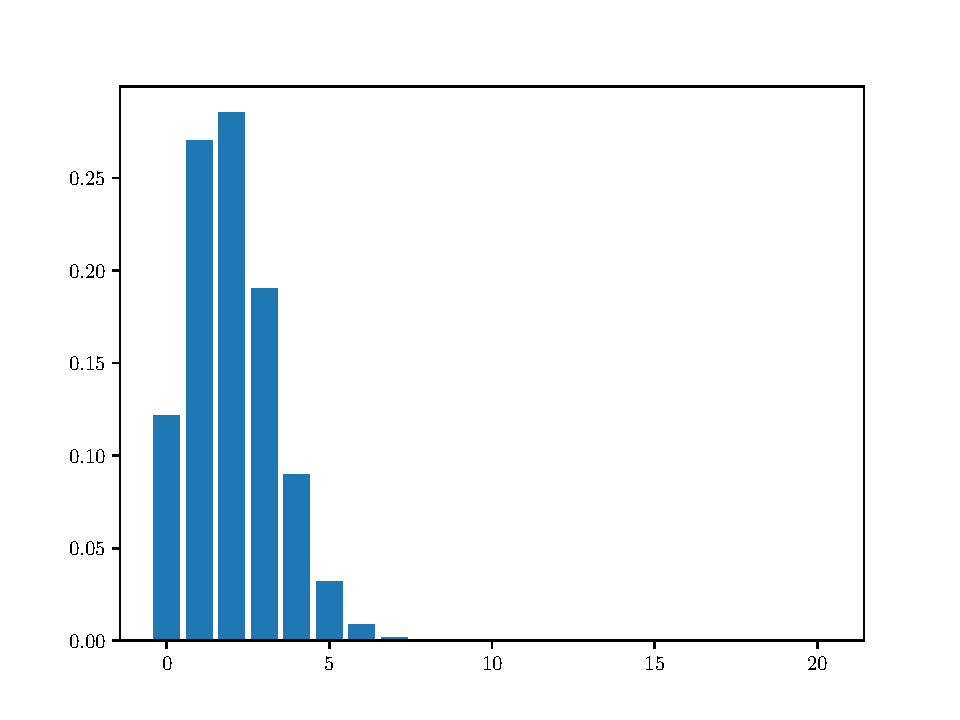
\includegraphics[width=\textwidth]{discrete/binomial/pmf_20_01.pdf}
		\caption{$B(20, 0.1)$}
	\end{subfigure}
	\begin{subfigure}[b]{0.45\textwidth}
		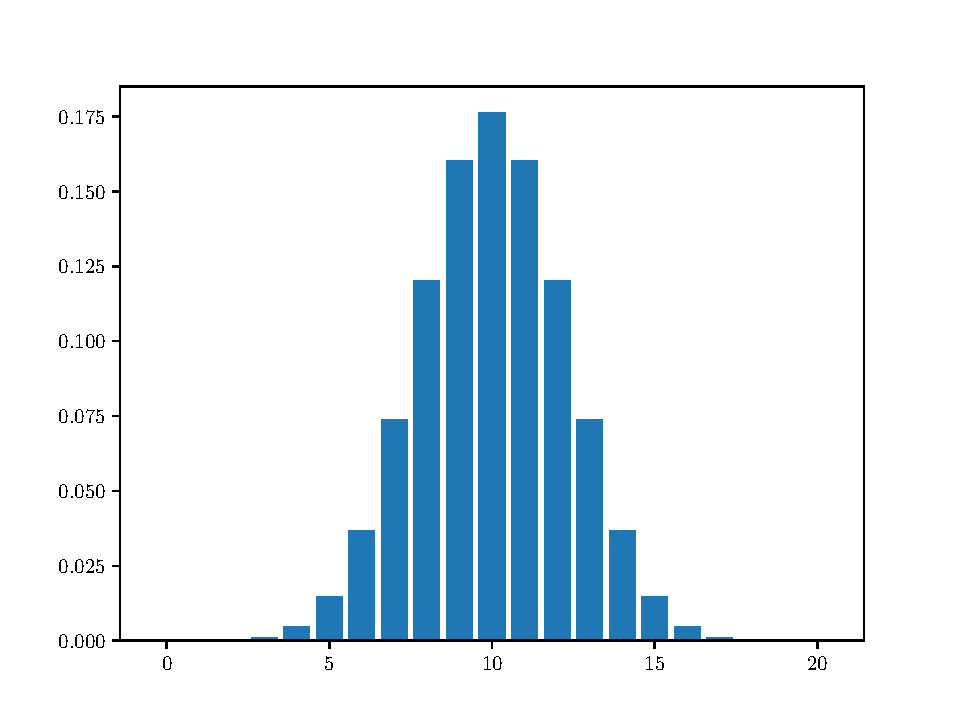
\includegraphics[width=\textwidth]{discrete/binomial/pmf_20_05.pdf}
		\caption{$B(20, 0.5)$}
	\end{subfigure}
	\begin{subfigure}[b]{0.45\textwidth}
		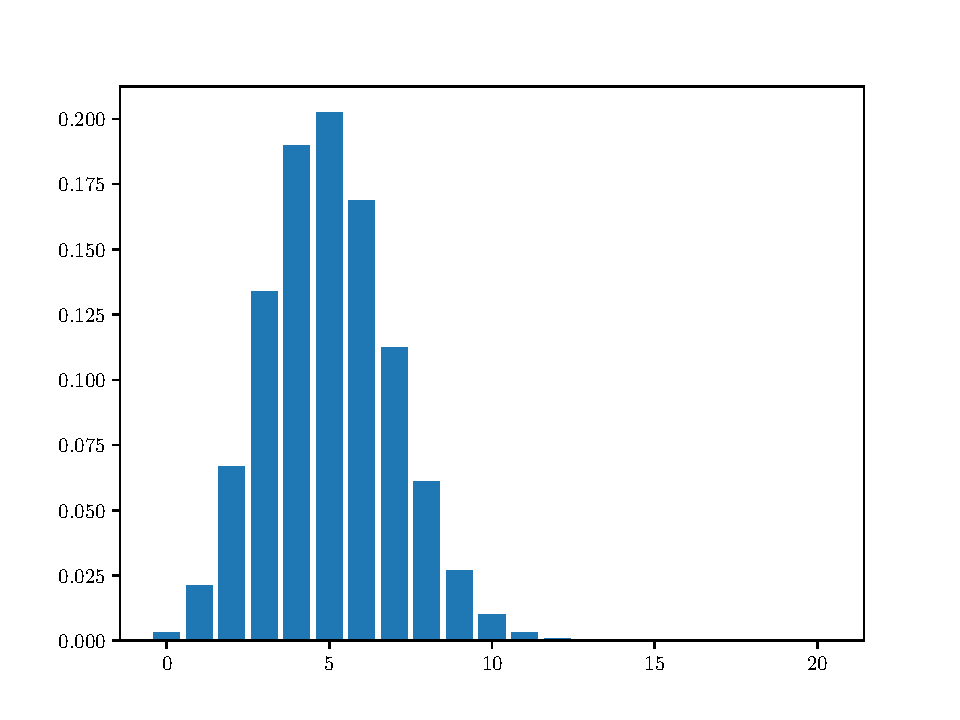
\includegraphics[width=\textwidth]{discrete/binomial/pmf_20_025.pdf}
		\caption{$B(20, 0.25)$}
	\end{subfigure}
	\begin{subfigure}[b]{0.45\textwidth}
		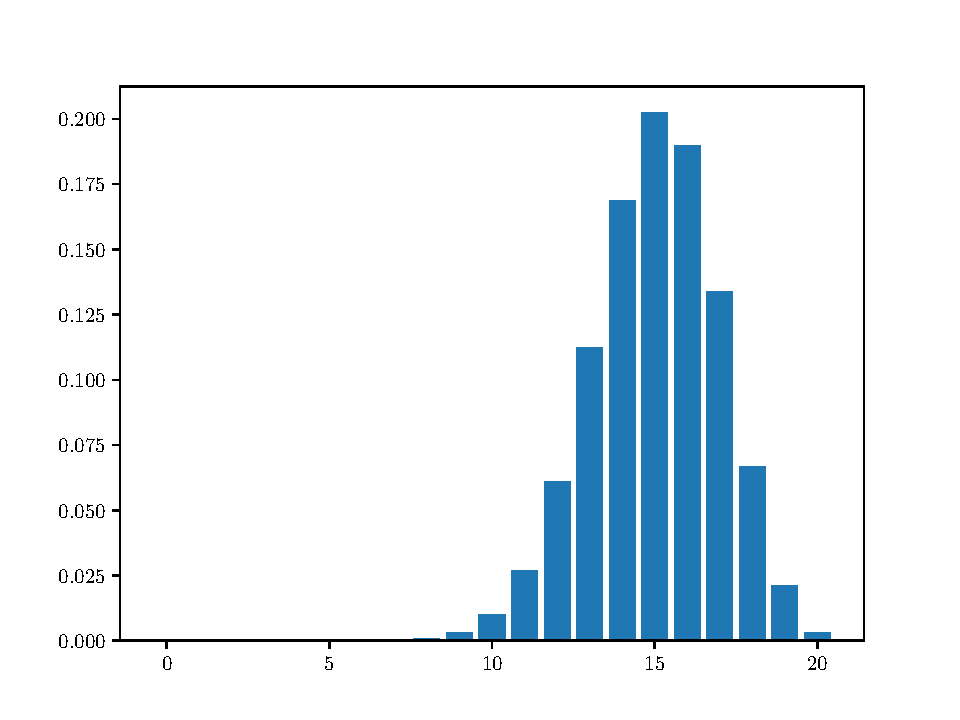
\includegraphics[width=\textwidth]{discrete/binomial/pmf_20_075.pdf}
		\caption{$B(20, 0.75)$}
	\end{subfigure}
	\begin{subfigure}[b]{0.45\textwidth}
		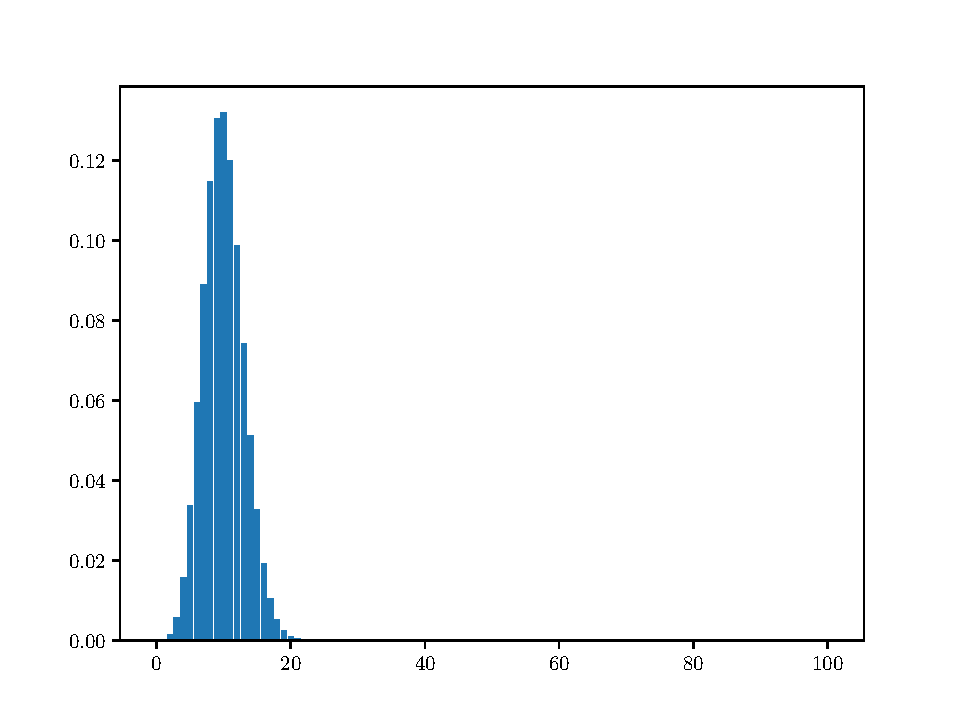
\includegraphics[width=\textwidth]{discrete/binomial/pmf_100_01.pdf}
		\caption{$B(100, 0.1)$}
	\end{subfigure}
	\begin{subfigure}[b]{0.45\textwidth}
		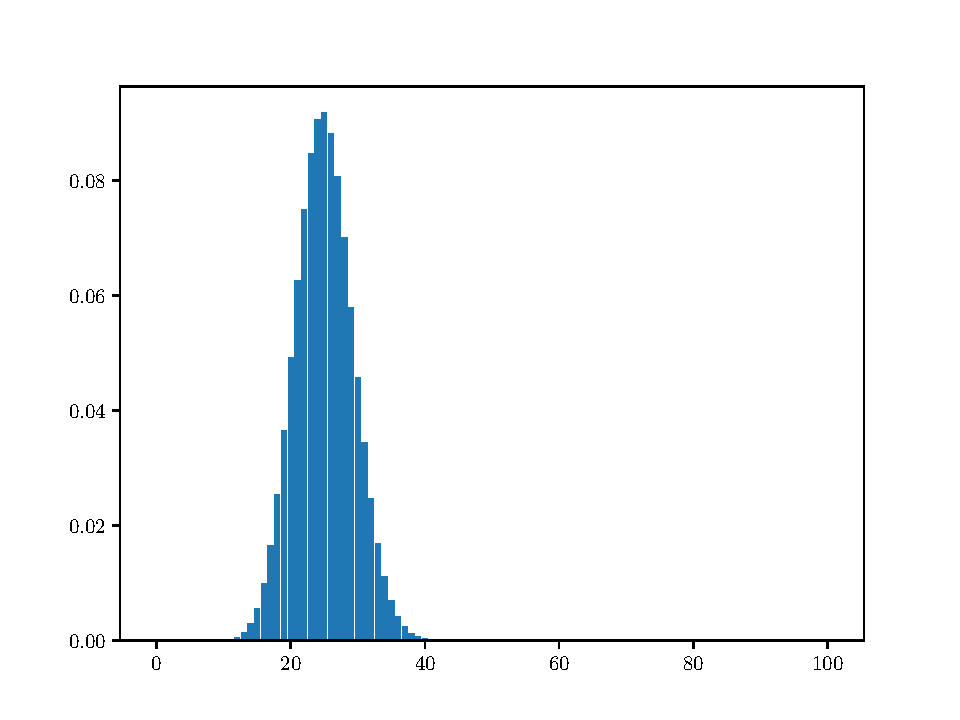
\includegraphics[width=\textwidth]{discrete/binomial/pmf_100_025.pdf}
		\caption{$B(100, 0.25)$}
	\end{subfigure}
	\caption{Binomial distribution}
\end{figure}

\begin{figure}[H]
	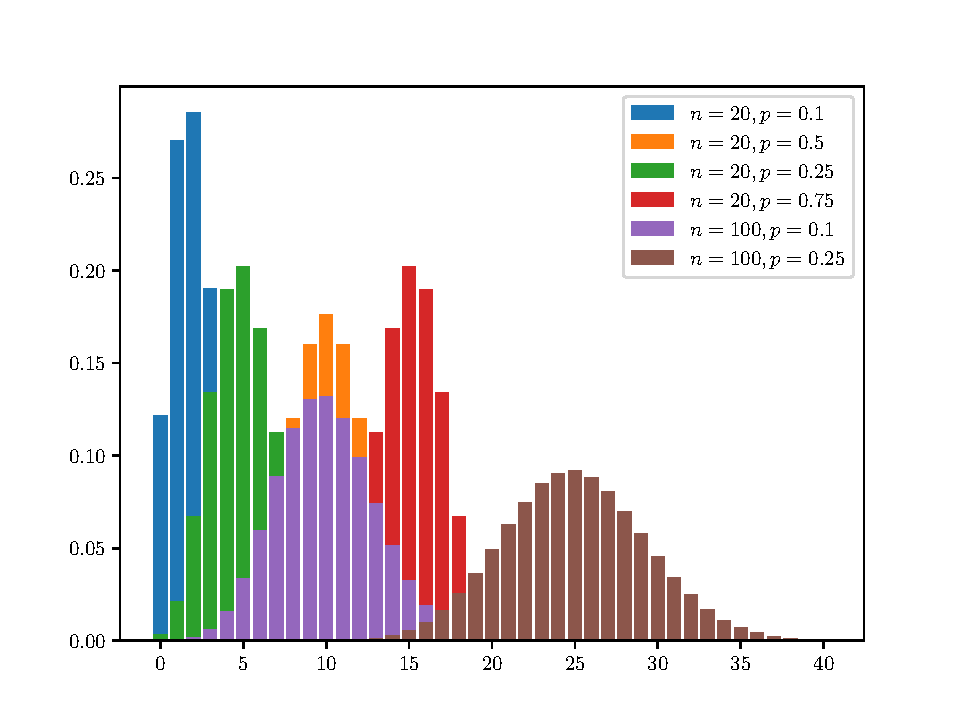
\includegraphics[width=\textwidth]{discrete/binomial/pmf_all.pdf}
	\caption{$P(X = k \mid n, p) = \binom{n}{k}p^{k}(1 - p)^{n - k}, \quad k = 0, 1, \ldots, n$}
\end{figure}

\subsection{Cumulative distribution function}
\[
	P(X \leq k \mid n, p) = \sum_{i = 0}^{k} \binom{n}{i}p^{i}(1 - p)^{n - i}, \quad k = 0, 1, \ldots, n
\]

\begin{figure}[H]
	\centering
	\begin{subfigure}[b]{0.45\textwidth}
		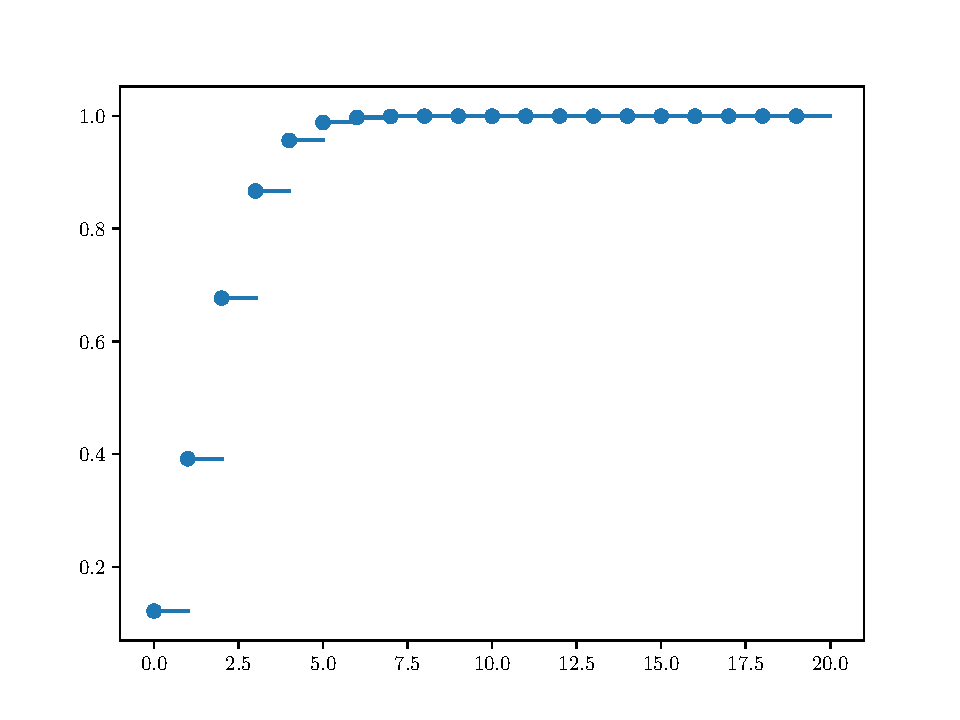
\includegraphics[width=\textwidth]{discrete/binomial/cdf_20_01.pdf}
		\caption{$B(20, 0.1)$}
	\end{subfigure}
	\begin{subfigure}[b]{0.45\textwidth}
		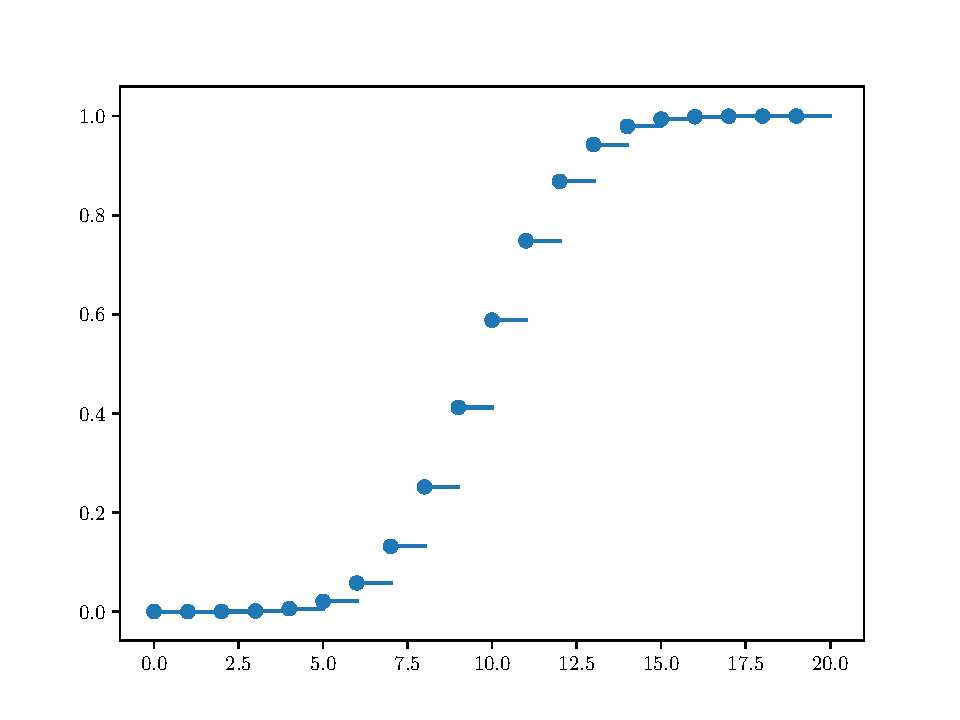
\includegraphics[width=\textwidth]{discrete/binomial/cdf_20_05.pdf}
		\caption{$B(20, 0.5)$}
	\end{subfigure}
	\begin{subfigure}[b]{0.45\textwidth}
		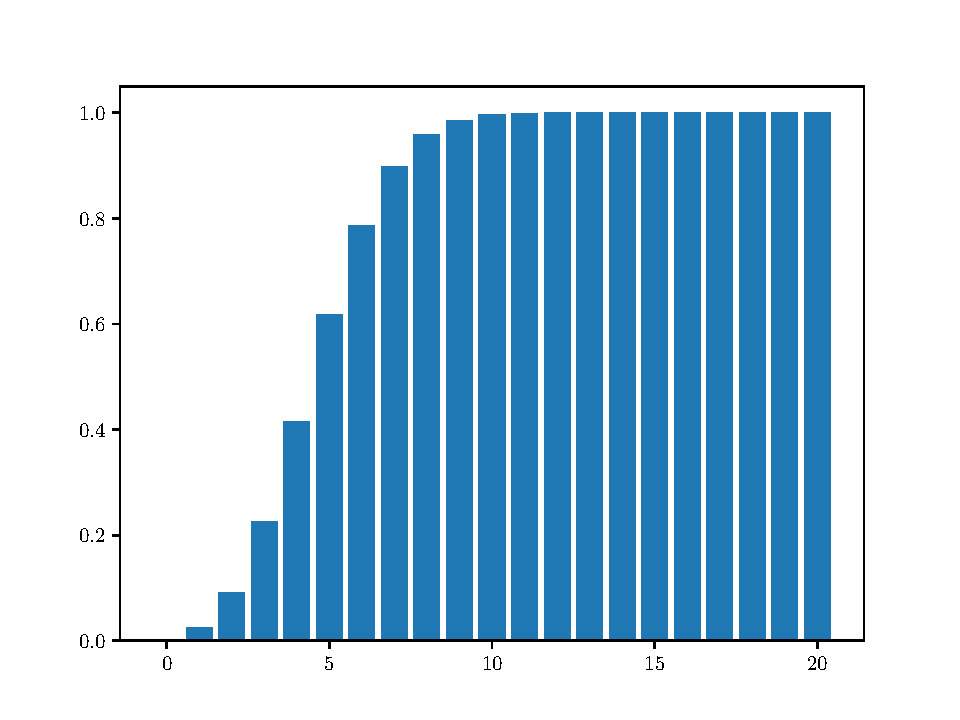
\includegraphics[width=\textwidth]{discrete/binomial/cdf_20_025.pdf}
		\caption{$B(20, 0.25)$}
	\end{subfigure}
	\begin{subfigure}[b]{0.45\textwidth}
		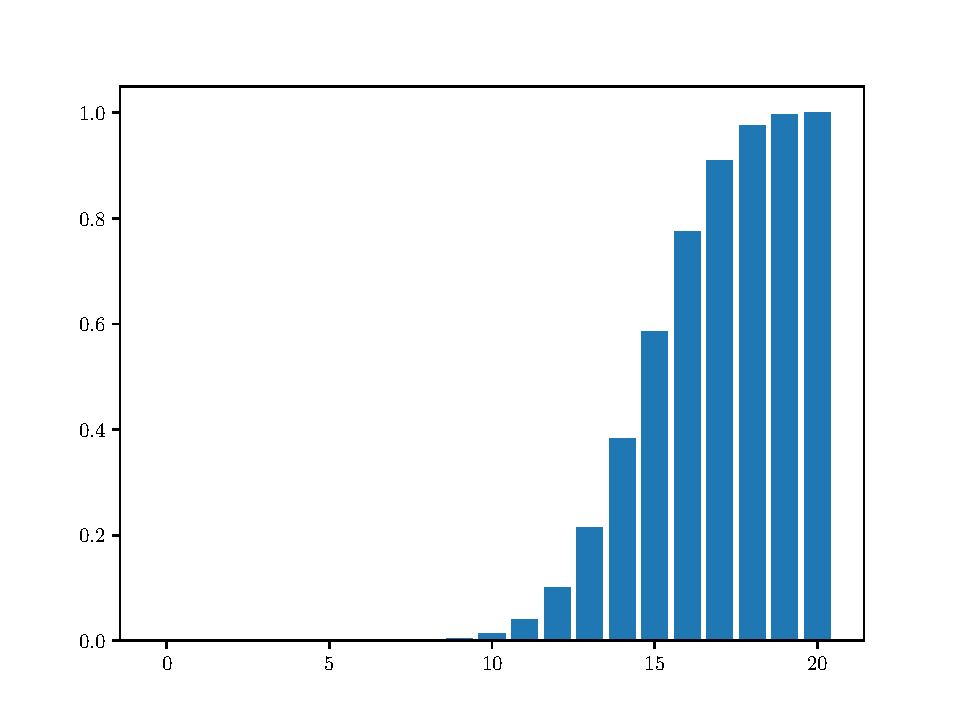
\includegraphics[width=\textwidth]{discrete/binomial/cdf_20_075.pdf}
		\caption{$B(20, 0.75)$}
	\end{subfigure}
	\begin{subfigure}[b]{0.45\textwidth}
		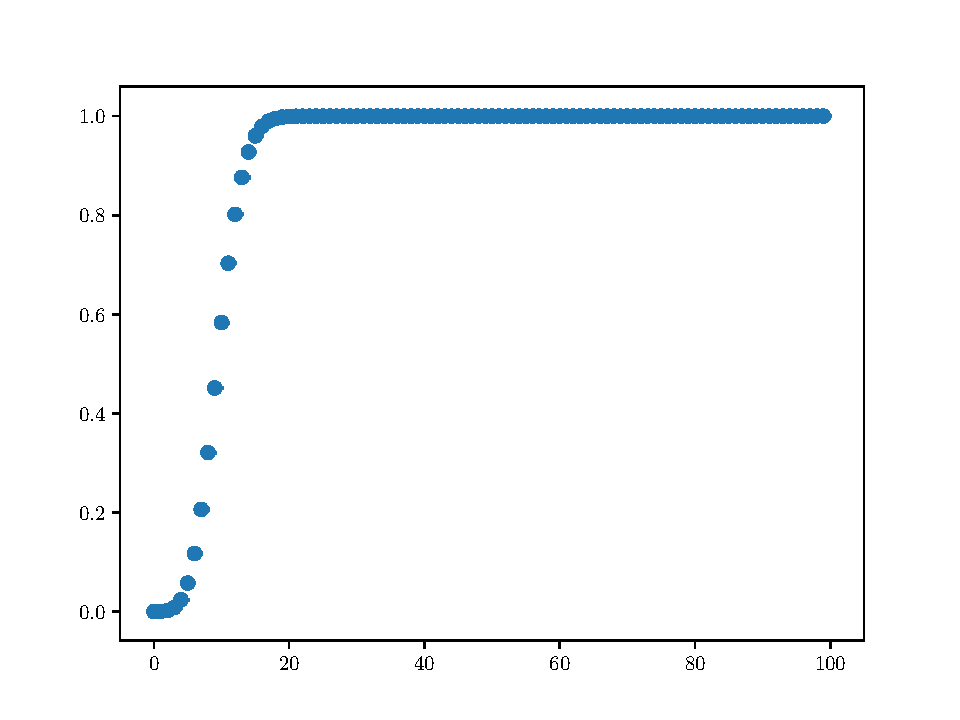
\includegraphics[width=\textwidth]{discrete/binomial/cdf_100_01.pdf}
		\caption{$B(100, 0.1)$}
	\end{subfigure}
	\begin{subfigure}[b]{0.45\textwidth}
		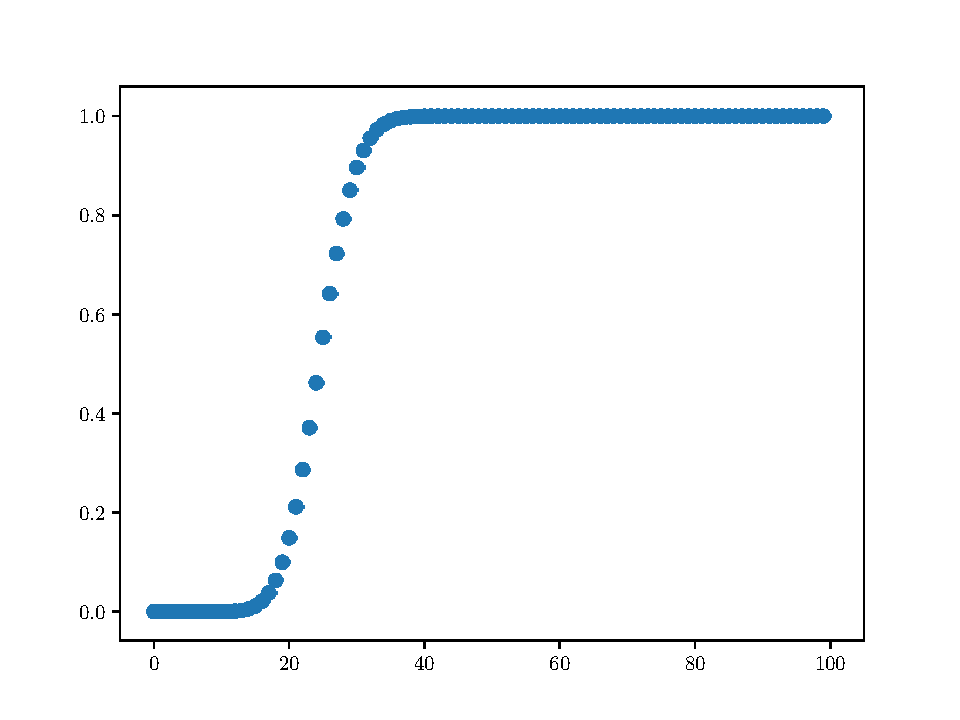
\includegraphics[width=\textwidth]{discrete/binomial/cdf_100_025.pdf}
		\caption{$B(100, 0.25)$}
	\end{subfigure}
	\caption{Binomial distribution}
\end{figure}

\begin{figure}[H]
	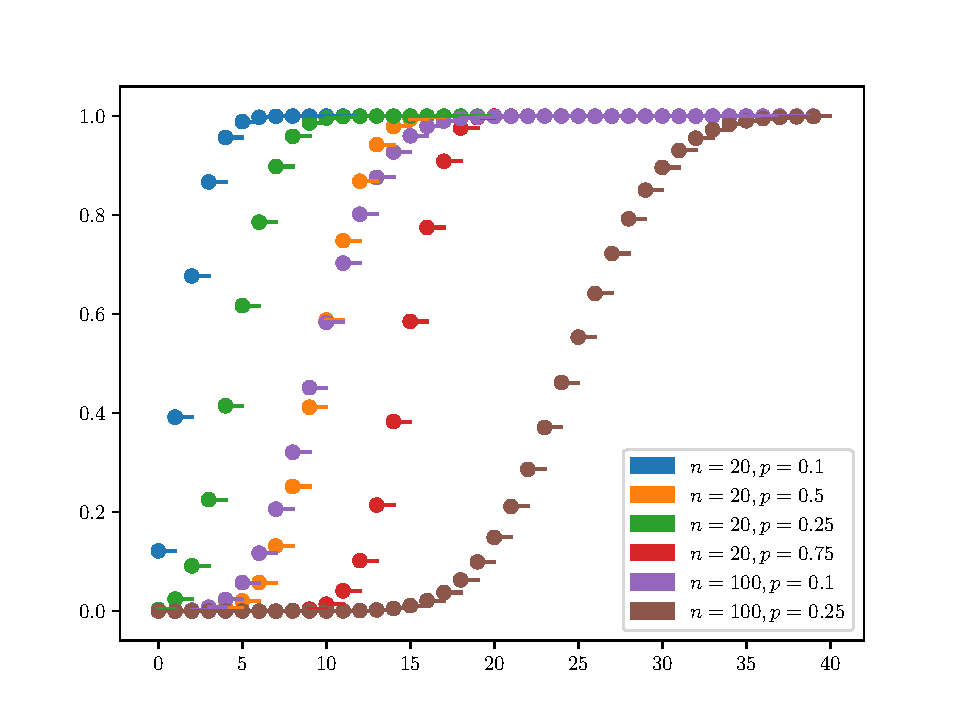
\includegraphics[width=\textwidth]{discrete/binomial/cdf_all.pdf}
	\caption{$P(X \leq k \mid n, p) = \sum_{i = 0}^{k} \binom{n}{i}p^{i}(1 - p)^{n - i}, \quad k = 0, 1, \ldots, n$}
\end{figure}

\section{Moments}

\begin{tabularx}{\textwidth}{s X}
	\hline
	Mean & $np$ \\\hline
	Variance & $np(1 - p)$\\\hline
\end{tabularx}

\section{Properties}
\begin{enumerate}
	\item Let $X_1, \ldots, X_m$ be independent random variables with $X_i \sim B(n_i, p), \ i = 1, 2, \ldots, m$. Then,
	\[
	\sum_{i = 1}^m X_i \sim B\left(\sum_{i = 1}^m n_i, p\right)
	\]
	\item Let $X_1, \ldots, X_m$ be independent Bernoulli$(p)$ random variables with success probability $p$. That is: $P(X_i = 1) = p, \ P(X_i = 0) = 1 - p, \ i = 1, \ldots, n$. Then,
	\[
	\sum_{i = 1}^m X_i \sim B\left(n, p\right)
	\]
\end{enumerate}

\section{Examples}
\begin{example}
	A fair die is rolled $n$ times.
	\begin{itemize}
		\item The probability of obtaining exactly one 6 is $n\left(\frac{1}{6}\right)\left(\frac{5}{6}\right)^{n - 1}$.
		\item The probability of obtaining no 6 is $\left(\frac{5}{6}\right)^n$.
		\item The probability of obtaining at least one 6 is $1 - \left(\frac{5}{6}\right)^n$.
		\item The number of trials needed for the probability of at least one 6 to be $\geq \frac{1}{2}$ is given by the smallest integer $n$ such that $1 - \left(\frac{5}{6}\right)^n \geq \frac{1}{2}$, so that $n \geq \frac{\log 2}{\log 1.2} \approx 3.8$.
	\end{itemize}
\end{example}


	
	\section{Poisson distribution}
	\subsection{Description}
The Poisson distribution expresses the probability of a given number of events occurring in a fixed interval of time or space if these events occur with a known constant mean rate and independently of the time since the last event. The Poisson distribution can also be used for the number of events in other specified intervals such as distance, area or volume.

For instance, an individual keeping track of the amount of mail they receive each day may notice that they receive an average number of 4 letters per day. If receiving any particular piece of mail does not affect the arrival times of future pieces of mail, i.e., if pieces of mail from a wide range of sources arrive independently of one another, then a reasonable assumption is that the number of pieces of mail received in a day obeys a Poisson distribution. Other examples that may follow a Poisson distribution include the number of phone calls received by a call center per hour, the number of decay events per second from a radioactive source, the number of visits to a website and the number of typographical errors per page in a book.

The Poisson distribution is an appropriate model if the following assumptions are true:

\begin{itemize}
	\item k is the number of times an event occurs in an interval and k can take values 0, 1, 2, ....
	\item The occurrence of one event does not affect the probability that a second event will occur. That is, events occur independently.
	\item The average rate at which events occur is constant.
	\item Two events cannot occur at exactly the same instant; instead, at each very small sub-interval exactly one event either occurs or does not occur.
\end{itemize}


\subsubsection{Probability mass function}
Let $X$ denote the number of events in a unit interval of time or in a unit distance.Then, $X$ is called the Poisson random variable with mean number of events $\lambda$ in a unit interval of time. The probability mass function of a Poisson distribution with mean $\lambda$ is given by
\[
 	f(k \mid \lambda) = P(X = k \mid \lambda) = \frac{e^{-\lambda} \lambda^k}{k!}, \ k = 0, 1, 2, \ldots
\]

\subsubsection{Cumulative distribution function}
\[
	F(k \mid \lambda) = P(X = k \leq \lambda) = \sum_{i = 0}^{k} \frac{e^{-\lambda} \lambda^i}{i!}, \ k = 0, 1, 2, \ldots
\]

The Poisson distribution can also be developed as a limiting distribution of the binomial, in which $n \rightarrow \infty$ and $p \rightarrow 0$ so that $np$ remains a constant. In other words, for large $n$ and small $p$, the binomial distribution can be approximated by the Poisson distribution with mean $\lambda = np$.

If the sample was drawn without replacement from a small finite population, the hypergeometric distribution should be used instead of the binomial.

\subsection{Moments}

\begin{tabular}{p{0.5\textwidth} p{0.5\textwidth}}
	\hline
	Mean & $\lambda$ \\\hline
	Variance & $\lambda$\\\hline
\end{tabular}

\subsection{Plots}
Poisson distribution is right-skewed, and the degree of skewness decreases as $\lambda$ increases.

\begin{figure}[H]
	\centering
	\begin{subfigure}[b]{0.45\textwidth}
		\includegraphics[width=\textwidth]{poisson/P2.png}
		\caption{$\lambda = 2$}
		\label{fig:P2}
	\end{subfigure}
	\begin{subfigure}[b]{0.45\textwidth}
	\includegraphics[width=\textwidth]{poisson/P3.png}
	\caption{$\lambda = 3$}
	\label{fig:P3}
	\end{subfigure}
	\begin{subfigure}[b]{0.45\textwidth}
		\includegraphics[width=\textwidth]{poisson/P5.png}
		\caption{$\lambda = 5$}
		\label{fig:P5}
	\end{subfigure}
	\begin{subfigure}[b]{0.45\textwidth}
		\includegraphics[width=\textwidth]{poisson/P10.png}
		\caption{$\lambda = 10$}
		\label{fig:P10}
	\end{subfigure}
	\begin{subfigure}[b]{0.45\textwidth}
		\includegraphics[width=\textwidth]{poisson/P20.png}
		\caption{$\lambda = 20$}
		\label{fig:P20}
	\end{subfigure}
	\begin{subfigure}[b]{0.45\textwidth}
		\includegraphics[width=\textwidth]{poisson/P30.png}
		\caption{$\lambda = 30$}
		\label{fig:P30}
	\end{subfigure}
	\caption{Poisson distribution}\label{fig:poisson}
\end{figure}

	
	
	%%%%%%%%%%%%%%%%%%%%%%%%%%%%%%%%%%%%%%%%%%%%%%%%%%%%%%%%%%%%%%%%%%%%%%%%%%%%%%%%%%%%%%%%%
	
\end{document}